\documentclass[]{article}

\usepackage{cite}
\usepackage{hyperref}
\usepackage[a4paper, total={6in, 10in}]{geometry}
\usepackage{graphicx}
\usepackage{amsmath}
\newtheorem{exmp}{Example}[section]
\graphicspath{ {images/} }



%opening
\title{Peerster - NoTrust\\
\large Team NoTrust}
\author{Raja Soufi, Pierre Thevenet}

\begin{document}

\maketitle

\begin{abstract}
The goal of our project is to extend Peerster's file sharing to include a reputation system, and include authenticity, confidentiality and integrity for files and messages. This will allow safer file transfer, and a fairer network.
\end{abstract}

\section{Goals and Functionalities}


\subsection{Authenticity, Integrity, Confidentiality and Web-of-Trust (Pierre)}

\subsubsection{Verifying the origin of a file}
\label{sec:goals-funcs-auth-integrity}
One of the goal is to add a way to verify the origin of a file. That is if a peer A receives a file created by C from the uploader B, A can verify if the true origin is indeed C. If it is, then it can accept the file, and if not, decide to discard the file and decrease the reputation of the uploader B (see \ref{sec:sig-based-rep}).

When requesting a download, the user will have to specify the origin of the file. Then the program will download it from the uploader (the destination of the file request) and if the uploader sends a correct file, it will accept it, otherwise drop it. \\

In the mean time, any file transfer in the network between a downloader A and uploader B will be signed by B so that A can verify that there is no man-in-the-middle. In fact the downloader does not necessarily expect that it comes effectively from B, but when our system will update the reputation of B according to its upload, hence A will need to verify if the file is true to what B sent. 

\subsubsection{Confidentiality with Private Messages}
Another goal is to improve Private Messages to be encrypted.

In the user's perspective, this will allow the possibility to send encrypted private messages to a (single) known destination. Because the peerster network is open to eavesdroppers, this will offer confidentiality on the content of a message in one-to-one communication. Similarly to a PGP encrypted email, only the content of the message will be encrypted.

This will be transparent to the user, all private messages will be limited to peers that obtained the public keys.

\subsubsection{Automated Web of Trust (AWOT)} 
The previous functionalities are implemented using public key cryptography. Usually the public keys are shared using a centralized PKI (Public Key Infrastructure), but our project will avoid this and implement a decentralized way to distribute public keys, based on the PGP "Web of Trust" model \cite{abdul1997pgp}.

Once the public keys are obtained, the previous functionalities (CIA) are straightforward, therefore our project is focused on the Automated Web of Trust rather than the possibilities offered by it, as they only serve as proofs of our working system.

Our system will build a table of relation between peers and public keys, and assign a trust level to each relation, representing the confidence that a particular public key belongs to a certain peer.

In summary our project also consist in a solution to the key validation and distribution problem. 

This enables all benefits from having public keys (e.g. authenticity, confidentiality...), while not relying on trusting a common authority. Hence we think it fits well in Peerster. \\

The user of our system will have to bootstrap the program with trusted public keys he knows from other users of Peerster, this will be the only action performed by the user in order to obtain public keys. The keyring will then automatically update itself and present a visualization.

We can imagine an extension in which the trust put in a particular peer depends on the user decision.

\begin{figure}[h]
	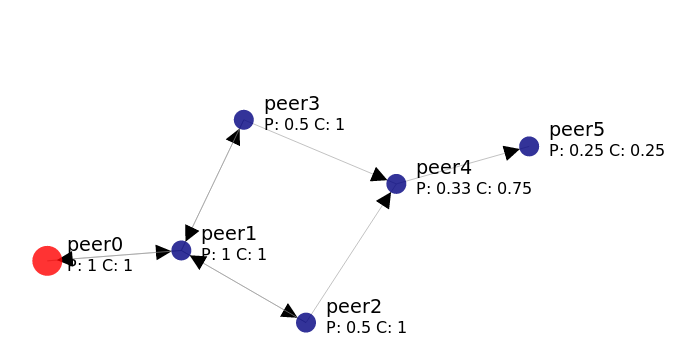
\includegraphics[width=\textwidth,height=\textheight,keepaspectratio]{keyring_example1}
	\centering
	\caption{Example of a Key Ring obtained with our implementation, see Fig. \ref{fig:pgp-key-ring} for explanations}
	\label{fig:keyring_ex1}
\end{figure}

However a visualization of the Web of Trust is given to the user (see Fig. \ref{fig:keyring_ex1}) (via the gui localhost:8080/keyring by default). This is to demonstrate the output of the AWOT system.

\subsection{Reputation (Raja)}
\label{sec:goals-funcs-rep}
The goal of having a reputation system in our implementation of Peerster is to improve the efficiency and security of the network.
Every peer A will compute a reputation for every other peer B based on three things:

\begin{itemize}
\item A's interactions with B
\item The communicated reputation of B from other peers, weighted by those other peers' reputations relative to A
\item The respective difference between the reputations of other peers communicated by B and those previously computed by A
\end{itemize}

Two types of reputation are computed for each peer. These are described below.

\subsubsection{Signature-Based Reputation}
\label{sec:sig-based-rep}
Every time A receives signed data originating from C delivered by B (note that B and C might be the same peer), A can check if the data delivered by B actually comes from C by means of Public Key Cryptography (as seen in \ref{sec:goals-funcs-auth-integrity}).
\\\\
If the data turns out to be authentic, then A will increase B's reputation, otherwise A will decrease it.
The amount by which A modifies B's reputation depends on the confidence level of C's public key that A holds, i.e. the degree to which we are confident that the public key we think is that of C is indeed that of C (see \ref{sec:related-work-wot}).
\\\\
In our implementation, we only update the signature-based reputation of a peer when checking signatures of file chunks.
It would have been possible to extend this to checking signatures of public key exchanges, but it was difficult to do for technical reasons specific to our implementation.

\subsubsection{Contribution-Based Reputation}
This type of reputation represents how much data B has delivered to A, relative to the total amount of data exchanged between the two.
Yet, more importance will be given to more recent interactions, as we will see in more detail in \ref{sec:background}.
\\\\
For this, A will recompute this type of reputation after every interaction with B based on the history of data flow between them.
This means that in a situation where both peers send data to each other in equal amounts, each of them will have a maximal reputation for the other, whereas in a situation where A sends much more data to B than the other way around, B will have a high reputation for A and A will have a low reputation for B.

\subsubsection{Usage}
Having reputations of other peers will mainly serve two purposes.
The first is related to choosing a confidence value for a public key association (see \ref{sec:design-arch-interop-rs-wts}).
The second, which affects more directly a peer's interaction with other peer's, is for choosing which peers to communicate with:
A peer with a high reputation is one that we know (at least recently) has been sending us authentic data regularly, and so it makes sense to prefer it over less reputable peer.
That is after all the main purpose of having a reputations system.
Other peers however may still be selected with low probabilities in order to "give other peers a chance" to increase their reputation and become more active.

\section{Related Work}

\subsection{CIA and Decentralized PKI}

\subsubsection{Confidentiality, Integrity and Authenticity}
This is a common problem, and solved using cryptography. Since in peerster we do not have a confidential channel to share a common key, we consider only public key cryptography. Two main solutions are RSA \cite{RFC8017} and elliptic curve cryptography (ECC). While ECC may be more promising, RSA is more reviewed.

\subsubsection{Decentralized PKI}
Decentralized PKIs already exist, and the main goal for them is to redistribute the roles of the certificate authorities in the common centralized PKI approach, and usually this mean not storing all public keys at the same place, and trusting the system. KeyChains \cite{morselli2006keychains} and \cite{aberer2005decentralised} are models for a decentralized PKI, the database of public keys are distributed which implies that a peer does not have every public keys, and that the retrieving of keys need more time than storing all keys in each system.

Implementing this in Peerster does not seem necessary, since every peer eventually save the entire set of active peers in the network (due to the specification). Our approach is to collect and save public keys for peers for each peerster client (total decentralization). Therefore this solution will save time for public key lookup (no decentralized database), at the cost of storage and network-redundant computations.

\subsubsection{Automated Web of Trust - AWOT}
\label{sec:related-work-wot}

The PGP Web of Trust Model \cite{abdul1997pgp} is a way to collect public keys using a social network, usually done in real life. For example, B signs the key of C, and gives the key to A, if A trusts B (which defines B as an "introducer"), A can trust that the given key indeed belong to C, and A can then signs the key of C. 

In Peerster we would want it to be automated, which is not the case in the common PGP model. 

One of the key point of the PGP model is the notion of trustworthiness of certificates and introducers. The trust of a certificate or introducer is decided by the user for each case, in Peerster we want it to be done automatically using the reputation and length of the certificate chain named "key ring" (see Fig. \ref{fig:pgp-key-ring}).

In the PGP model the level of trust is discrete (e.g. 'marginal', 'complete', 'untrustworthy' ...) but the meaning of this levels are not explicit and left for interpretation. We will therefore extend this model with a level of trust representing a 'probability' of confidence in the association key-peer. This idea is described in \cite{haenni2007new}, which is a natural extension to the PGP model and seems reasonable.

\begin{figure}[h]
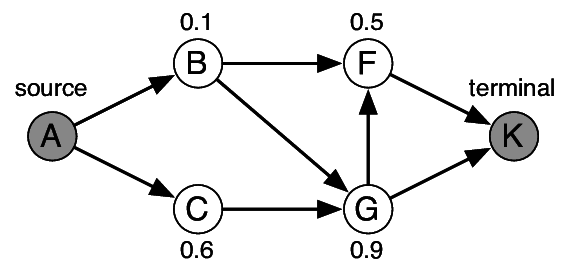
\includegraphics{pgp-key-ring}
\centering
\caption{Example of a PGP Key Ring}
\label{fig:pgp-key-ring}
Source : \cite{haenni2007new}

Here each vertex is a peer, and each edge Y $\rightarrow$ Z means that Y signed the key for Z.
Each figure associated with a vertex Z  correspond to the trust level given in the public key, we will name it the probability of Z, $Pr(Z)$.
\end{figure}

\subsection{Reputation}
This is also a common problem, and different variations of a common approach have been studied in order to manage reputation in a distributed system while minimizing the possibilities for malicious peers to abuse the reputation system in order to gain reputation and do malicious activity.
\\\\
For instance, \cite{gupta2003reputation} computes a global reputation for each peer, which uses local reputation values assigned to it by other peers, weighted by those peers' global reputations.
\cite{despotovic2006p2p} takes a similar approach but computes a trustworthiness of a node by doing a weighted average of the experiences of the nodes that interacted with that node.
Another interesting approach is that of \cite{zhou2007powertrust}, in which each node is rated with a global reputation score which is based on weighted local scores from neighbors.
\\\\
Our implementation will follow a similar approach, but will be slightly simpler for the sake of this project:
Each peer A computes a local reputation for every other peer B, as we saw in \ref{sec:goals-funcs-rep}.
Yet, from time to time A will ask its $n$ most reputable peers for their reputation tables, and will use the reputations in those tables, wheighted by the reputations of those $n$ peers, to update its reputation table.
Furthermore, when it receives the reputation tables of its $n$ most reputable peers, A will compute some sort of Hamming distance between each peer's table and its own table and use that distance to update that peer's reputation.
\\
However, when updating peers' reputation values with either of these two methods, the highest weight will still be given to the previous value we are updating.
This way, values introduced by peers will only introduce small variations to the reputations in A's table, which will still be mostly controlled by A's own interactions with other peers.

\section{Background}
\label{sec:background}

\subsection{Cryptography}
Since our project will be written in go, we will use standard cryptographic libraries for go. We will use RSA \cite{RFC8017}.

\subsection{Web of Trust}
\label{sec:web-of-trust-spec}
We will implement the idea of \cite{haenni2007new}.

\subsubsection{Key exchange}

All peers are given fully trusted public keys from the users' input.
These keys are then signed, and sent alongside the key itself as a special Rumor Message, so that any peer in the network will eventually receive it.

Sometimes a signature can be received from an unknown peer, therefore the key cannot be verified. In this case, such received messages are stored and periodically checked until enough keys have been received.

\subsubsection{Algorithm}
\label{sec:wts-algo}
In details, consider the network in Fig.\ref{fig:pgp-key-ring}. For validating the public key of K, we follow the steps : \\

1. Compute the shortest paths from A to K \\\\
Here the shortest paths are $paths = \{(A,B,F,K), (A,B,G,K), (A,C,G,K)\}$\\

2. Then compute the "probability" $p$ of the set of paths : \newline
Define, for distinct peers $A_1,...,A_n$ and path $path = (A_1,...,A_n)$, $Pr(path) = \prod_{i = 1}^{n} Pr(A_i)$, i.e. the confidence put on each peer is independent from the confidence put on any other peer. \\
$Pr(paths)$ is computed using the inclusion exclusion formula over the shortest paths. \\\\


\begin{multline}
Pr(paths) = Pr((A,B,F,K)) + Pr((A,B,G,K)) + Pr((A,C,G,K)) \\
		    - Pr((A,B,F,K,G)) - Pr((A,B,F,K,C,G)) - Pr((A,B,G,K,C)) \\
		    + Pr((A,B,F,K,G,C)) \\
		  = 0.581
\end{multline}

3. If $p > \lambda$ accept the key, else reject it. \\\\
Here, if $\lambda = 0.6$, reject the key : the certificate chain may be too long, or the confidence on the peers too low.\\


In short, the more shortest paths from source to the terminal and the lest hops in these paths, the higher the confidence. Adding to that the confidence level for each hop, and we get this algorithm.

\subsubsection{Parameters}
\label{sec:parameters}
$\lambda$ is the acceptance threshold. We will fix it to 0 for simplicity, meaning that we prefer to use cryptography with uncertain peer rather than not communicating with it. \newline
The 'probabilities' assigned to each peers are computed using the reputation system and the distance from the source in the graph. We will use $min(2 \times rep_A, \frac{1}{d})$ as the probability of $A$, where $rep_A$ is the current reputation of $A$ and $d$ is the distance from this peer in the key ring. This way we enforce the distance and the reputation to be acceptable.

\subsection{Reputation}
\label{sec:rep-spec}
Most of the techniques used for this part have a rather mathematical aspect to them than algorithmical.

\subsubsection{Signature-Based Reputation}
For this type of reputation, we will use a simple formula with a nice property:

\begin{equation}
    \label{eq:sig-rep}
    RS_n = 
    \begin{cases}
        RS_{n-1} + f_+(c),       & \text{if the received data is authentic}
        \\
        \frac{RS_{n-1}}{f_-(c)}, & \text{otherwise}
    \end{cases}
\end{equation}

\noindent
Where $RS_n$ is the signature-based reputation of peer B that sent the data at some point n, $c$ is the confidence level of B's public key association, and $f_+(c)$ and $f_-(c)$ are functions of $c$ that are used to control the impact of this new interaction on B's reputation based on the confidence level $c$.
These can be chosen later on, but the important idea here is that behaving non-maliciously will only increase a peer's reputation linearly, while behaving maliciously will decrease it exponentially.
This somehow makes it a lot harder for malicious peers to do a significant amount of malicious activity while still interacting in the system with a good reputation.

\subsubsection{Contribution-Based Reputation}
For this type of reputation, we will use an Exponentially Weighted Moving Average:

\begin{equation}
    \label{eq:contr-rep}
    RC_n =
    \begin{cases}
        RC_initial,                                     & \text{if}\ n = 1
        \\
        \alpha \cdot S + (1 - \alpha) \cdot RC_{n - 1}, & \text{otherwise}
    \end{cases}
\end{equation}

\noindent
Where $RC_n$ is the contribution-based reputation of peer B that sent/received data at some point n, $RC_initial$ is an initial contribution-based reputation constant that is assigned to all peers at the beginning, $\alpha$ is the main parameter of the Moving Average, and $S$ is $1$ if B was the sender during this interaction and $0$ if it was the receiver.
\\\\
Note that the value of $\alpha$ determines how much weight we give to the current interaction and to the history of interaction.

\section{Design and Architecture}

Our project is built on the common Peerster, adding to it our modules. In particular the transfer of messages (broadcast and private) and file sharing are the most important features our system will use. We disabled nat traversal and file search functionnalities for simplicity.

\subsection{Systems}
Our system can be divided into two different but interconnected systems : the Reputation System (RS) and the Automated Web of Trust system (AWOTS). \newline
Figure \ref{fig:no-trust-arch} illustrates the overall structure of the system and the interactions between the two subsystems.

\begin{figure}[h]
	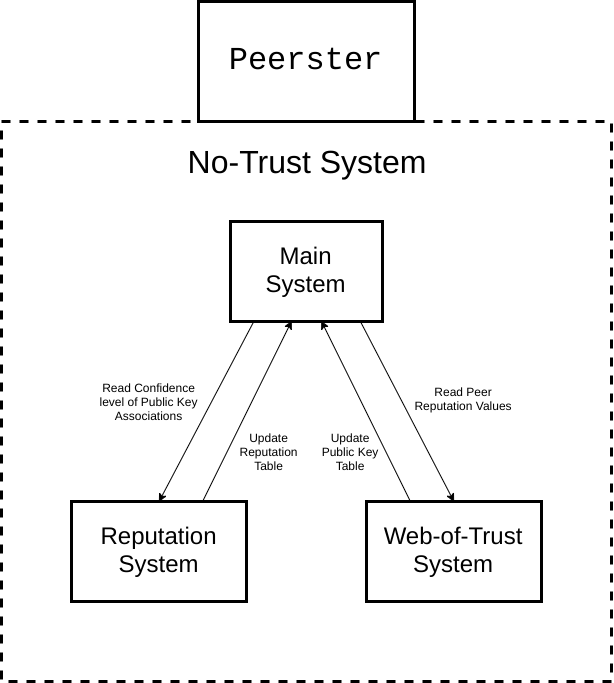
\includegraphics[width=50mm]{no-trust-arch}
	\centering
	\caption{General architecture of the No-Trust system}
	\label{fig:no-trust-arch}
\end{figure}

\noindent
Pierre will do the Automated Web of Trust System, and Raja will do the Reputation system.

\subsubsection{Automated Web of Trust System}
This system will be responsible for updating a table in the Main System which will include $(id, k^{pub}_{id}, confidence_{id})$ for each known peer with identifier $id$, where $k^{pub}_{id}$ is the (trusted) public key of this peer, and $confidence_{id}$ is the confidence level put in the association $id \leftrightarrow k^{pub}_{id}$. \\
This table will be used for getting the public keys of the different peers, and the confidence values will be used for the Reputation System and cryptographic functions. \\

At startup, trusted peers with their corresponding public keys will be given. Then each peer will start to sign its neighbors' public keys, and send the keys with signature to everyone in the network via rumor messages. \\
When receiving a signature and a key, the AWOTS will update the key ring, and run the algorithm described in \ref{sec:wts-algo} if enough information. If the key is accepted, then the peer is added to the trusted peers, and then continue the process.
This steps will add more and more public keys to the table. 

Periodically the system will update the confidence levels in the table by running the same algorithm on the already acquired keys. \\

Problems may arise, like collision of two different keys for the same peer (same identifier), in this case the system will pick the biggest subset of minimum paths to the identifier with the same key and "forget" the other paths (having different keys). Therefore for a key to be accepted, it has to be part of the maximum number of minimum paths. A more detailed discussion is given in \ref{sec:example-collision}.

\subsubsection{Reputation System}
This system will be responsible for updating a separate table in the Main System which will include $(id, RS_n, RC_n)$ where $RS_n$ and $RC_n$ are the signature-based and contribution-based reputations respectively, as we saw in \ref{sec:rep-spec}.
This table will be used both to choose peers to interact with as well as to compute confidence levels in the Web of Trust System.
\\\\
Given that the very definition of reputation relies on history, all peers will have the same initial reputation, which seems like the most natural state to start the system with.
Then, as we saw earlier, the two reputation values (in each entry of the table) will be updated on every interaction with the corresponding peer, as well as periodically when peers ask their most reputable peers for their tables.
\\
Obviously, we might get completely invalid reputation values from a peer (e.g. outside the set bounds), in which case we might consider penalizing that peer even more.

\subsubsection{Main System}
The main system will be implemented with base the common Peerster project. \\
We will add features like confidentiality, integrity and authenticity to the messages and files, in this main module. The difference in the messages will be set by some flags, which will indicate if the message is an encrypted file or has a signature. Then the messages can be demultiplexed according to this flags.

As discussed earlier, the reputation table will be used to choose a peer to interact with, for example when a peer wants to ask for the public key of another peer, or when it wants to send a status packet to update its rumors.
\\
Highly reputable peers will be chosen with a very high probablity. For instance, assuming the table is sorted somehow based on the reputation values, we might select a peer from the upper half of the table with probability $0.9$ and from the lower half with probability $0.1$, and recursively select a half with probabilities that are more and more balanced with every iteration.
This will occasionally give low reputable peers a chance to make a "come back" and contribute in the system.

\subsection{Systems interoperability}

\subsubsection{Use of WTS for RS}
The output of the Web-of-Trust system will be used when updating the signature-based reputations of peers (hence the name).
The confidence level for each public key association is a perfect variable to be used as a liability measure:
If we're not completely sure that the public key we have for a peer is indeed his public key, it wouldn't be completely fair to penalize him as much as if we were 100\% sure of his public key.

\subsubsection{Use of RS for WTS}
\label{sec:design-arch-interop-rs-wts}
The reputation system will be helpful for determining the probabilities as discussed in \ref{sec:parameters}, by providing the signature-based reputation (see \ref{sec:sig-based-rep}). This reputation gives information about the honesty of a peer : if this peer sent badly signed packets or not. Therefore we will assign the confidence level of each peer in function of its reputation.

\subsubsection{Use of WTS for the cryptographic functionalities}
The WTS will provide the public keys needed for encryption and verification of signatures.

\section{Evaluation Plan}

\subsection{Cryptography}
\label{sec:crypt-test}
We will verify correctness of the cryptographic functionnalities (confidentiality, integrity and authentication) with some cases (e.g. sending well/badly signed files, sending encrypted messages and decoding them at receiver, ...), only to check that the standard libraries have been well implemented in our project. We will not evaluate the "crypto" and "crypto/rsa" libraries and will expect them to be correct.

\subsection{Web of Trust}
To measure the correctness and performance of our key distribution system (WTS), we will create a scenario with a network of Peerster nodes, and follow the updates of the key ring of each node, checking the time at which the ring stops updating, and checking the correctness of the ring. The state of the WTS system is the key ring, therefore checking the key ring is enough to evaluate the correctness of the system. The performance will be tested, but because of the nature of Peerster and the possibility of network bottlenecks, we will check that the key ring is complete after a reasonable amount of time. Moreover since the public keys are obtained via this system, testing in \ref{sec:crypt-test} will effectively test if the WTS works.

Results

On a local setup, with a network of seven nodes, convergence is attained in less than 10 seconds in mean. We think this is correct for our project, and in accordance with the tests we were given for the previous stages. Looking at the algorithm, the overhead may not scale well if the number of minimum paths becomes too large, but this is an optimization problem and not in the scope of our project.

\subsection{Reputation}
To evaluate the reputation system, we will follow a similar approach as for the rest of the system.
We will run the system in a controlled environment where we send particular specific messages that we know should trigger certain changes in the reputation tables in order to check that these changes are actually happening.
\\\\
We will check for example that signature-based reputations are being decreased exponentially when receiving inauthentic data and increased linearly otherwise (as described by equation \ref{eq:sig-rep}).
We will also check that the moving average for contribution-based reputation discards history more and more over time (as described by equation \ref{eq:contr-rep}).
Finally, we will make sure that a peer chooses in most cases its most reputable peers before initiating interactions such as rumor mongering.

\section{Discussions}

\subsection{Automated Web Of Trust}

\subsubsection{Example and Collisions of keys}
\label{sec:example-collision}
Collision of two different keys for the same peer (same identifier) is possible. In this case the system will pick the biggest subset of minimum paths to the identifier with the same key and "forget" the other paths (which have different keys). Therefore for a key to be accepted, it has to be part of the maximum number of minimum paths.

\begin{exmp}
	
	In this scenario, we see a simplified keyring with the only important edges from A's perspective. We are interested in G's public key.
	The minimum paths in Fig \ref{fig:keyring_good1} are (we do not consider the source nor the terminal since they do not count in the computations) :
	
	\[ { \{B,D\}, \{B,E\}, \{C,F\}  } \]

	\begin{figure}[h]
		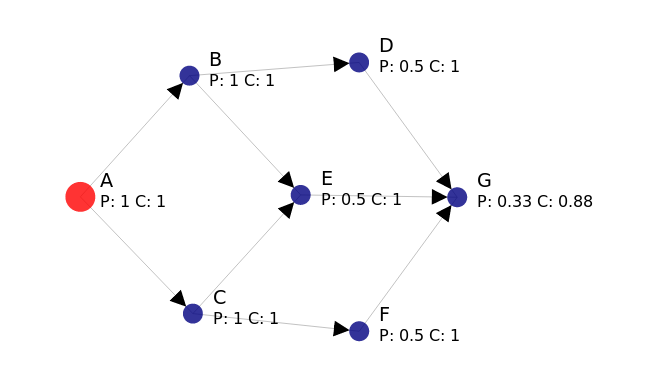
\includegraphics[width=\textwidth,height=\textheight,keepaspectratio]{keyring-good1}
		\centering
		\caption{Key Ring with all good nodes}
		\label{fig:keyring_good1}
	\end{figure}
	
	However the minimum paths in Fig \ref{fig:keyring_bad1} are :
	
		\[ { \{B,D\}, \{B,E\}  } \]
		
	
	The system do not consider the path $\{C,F\}$ anymore because $F$ sent a key different from $D$ and $E$ and therefore is no longer in the same set of paths.
	
	We can observer the confidence in G's key dropping from 88\% to 75\% due to $F$ no longer being considered.	
	
	Of course if $E$ becomes malicious too and advertises the same key as $F$, we will trust $E$ and $F$ because they become majority.
	
	If $E$ is malicious but sends a different key than $F$, the system will choose one of those three keys.
	
	\begin{figure}[h]
		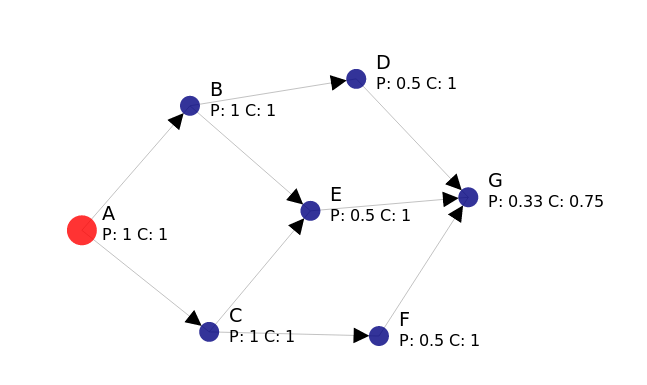
\includegraphics[width=\textwidth,height=\textheight,keepaspectratio]{keyring-bad1}
		\centering
		\caption{Key Ring with malicious F node}
		\label{fig:keyring_bad1}
	\end{figure}

	This setup can be reproduced using the tests given with the source code.

\end{exmp}

\subsection{Reputation System}
  The behavior of contribution-based reputations seems a little bit undeterministic in some cases and does not always react the way we expect it to.
  \\
  For instance, if we send a lot of successive rumors from one peer, we might think that its contribution-based reputation will increase dramatically in all peers directly connected to that peer.
  However, that does not seem to be the case, and we can observe that all reputations drop at that point.


\bibliography{references}{}
\bibliographystyle{plain}

\end{document}
